\documentclass[fontset=windows]{article}
\usepackage[margin=1in]{geometry}%设置边距,符合Word设定
\usepackage[UTF8]{ctex}
\usepackage{setspace}
\usepackage{amsmath}
\usepackage{amssymb}
\numberwithin{figure}{section}
\usepackage{array}
\usepackage{lipsum}
\usepackage{float}
\usepackage{graphicx}%插入图片
\usepackage[dvipsnames]{xcolor}
\usepackage{authblk}
\usepackage{listings,matlab-prettifier}
\lstset{
	language=Matlab, % 设置代码语言为Matlab
    basicstyle=\ttfamily, % 设置字体为等宽字体
    numbers=left, % 行号在左边显示
    numberstyle=\tiny, % 设置行号字体大小
    stepnumber=1, % 行号递增步长
    numbersep=5pt, % 行号到代码的距离
    backgroundcolor=\color{gray!10}, % 设置代码的背景颜色
    showspaces=false,
    showstringspaces=false,
    showtabs=false,
    frame=single, % 设置代码框
    rulecolor=\color{black},
    tabsize=2,
    breaklines=true,
    breakatwhitespace=true,
    title=\lstname,
	keywordstyle=\bfseries\color{NavyBlue},
	morekeywords={var,};
	emphstyle=\bfseries\color{Rhodamine}, % 强调词样式设置
    commentstyle=\itshape\color{black!50!white}, % 设置注释样式,斜体,浅灰色
    stringstyle=\bfseries\color{PineGreen!90!black}, % 设置字符串样式
	columns=flexible,}
\graphicspath{{Figures3/}}%文章所用图片在当前目录下的 Figures目录

\usepackage{hyperref} % 对目录生成链接,注:该宏包可能与其他宏包冲突,故放在所有引用的宏包之后
\hypersetup{colorlinks = true,  % 将链接文字带颜色
	linkcolor=black, % 将链接文字黑色
	bookmarksopen = true, % 展开书签
	bookmarksnumbered = true, % 书签带章节编号
	} % 作者
\bibliographystyle{plain}% 参考文献引用格式

\renewcommand{\contentsname}{\centerline{目录}} %经过设置word格式后,将目录标题居中

\title{\heiti\zihao{2} 《统计信号处理》第二教学单元研讨题}
\author{杨 鼎,韦可雷,高司博,高涵博}
\date{}

\begin{document}
\maketitle
\thispagestyle{empty}

%\begin{abstract}
%	\lipsum[2]
%\end{abstract}

%\tableofcontents
%\setcounter{page}{0}
%\newpage

\section{第一题}
获得贝叶斯估计的准则有哪些?先验信息通常如何确定?什么是无信息先验?以观测模型\(z=A+w\)为例,
其中观测噪声\(w\sim \mathcal{N}(0,\sigma^2)\)且与A相互独立。如果对待估参数A没有更多的知识,
你认为可以如何处理?如果要估计的参数是\(\beta=e^A\)时,情况又如何?


\subsection*{(1)获得贝叶斯估计的准则有哪些?}

获得贝叶斯估计的准则有最大后验概率、最小均方(MMSE,也称条件均值)、条件中位数估计、
线性最小均方估计

\subsection*{(2)先验信息通常如何确定?}

先验信息通常建立在物理约束规律之上。一般,如果待估计量知道其取值范围,
则待估计量先验概率密度选择这个范围上的均匀分布。

\subsection*{(3)由什么是无信息先验?}

无信息先验是对于确定性参数利用贝叶斯方法估计时(确定性参数估计通常不采用贝叶斯估计而采用最大似然估计),
先验PDF不含信息量,不向问题增加任何信息。

\subsection*{(4)以观测模型\(z=A+w\)为例,
	其中观测噪声\(w\sim \mathcal{N}(0,\sigma^2)\)且与A相互独立。如果对待估参数A没有更多的知识,
	你认为可以如何处理?如果要估计的参数是\(\beta=e^A\)时,情况又如何?}

如果参数A没有任何没有更多信息,采用最大似然估计,或采取无先验信息的贝叶斯估计。

采取最大似然估计得到\(\hat{A}=\overline{\mathbf{x}}\),由似然函数不变性得到
\(\hat{\boldsymbol{\beta}}=e^{\overline{\mathbf{x}}}\)。

\section{第二题}
贝叶斯估计器与后验分布\(p(A|\mathbf{z})\)有什么关系?是否可以用后验方差来评价最小均方误差估计器的性能?
参数A的先验方差、后验方差以及贝叶斯最小均方误差之间有无关系?

\subsection*{(1)贝叶斯估计器与后验分布\(p(A|\mathbf{z})\)有什么关系?}
由于A是一个随机变量,所以期望运算是对联合PDF\(p(\mathbf{z},A)\)求取的,这是贝叶斯估计与经典估计本质上的不同,
贝叶斯均方误差定义为:
\begin{align*}
	Bmse(\hat{A})=\int\int(A-\hat{A})^2 p(\mathbf{z},A)d\mathbf{z}dA
\end{align*}

依据贝叶斯原理,我们有:
\begin{align*}
	p(\mathbf{z},A)=p(A|\mathbf{z})p(\mathbf{z})
\end{align*}
所以贝叶斯均方误差由可以写成:
\begin{align*}
	Bmse(\hat{A})=\int \left[\int (A-\hat{A})^2 p(A|\mathbf{z})dA\right]p(\mathbf{z})d\mathbf{z}
\end{align*}
又由于对所有的\(\mathbf{z}\)而言都有\(p(\mathbf{z})>0\),如果括号内的积分对每个\(\mathbf{z}\)都最小,
那么贝叶斯均方误差将达到最小:
\begin{align*}
	\frac{\partial}{\partial \hat{A}}\int (A-\hat{A})^2 p(A|\mathbf{z})dA
	 & =\int \frac{\partial}{\partial \hat{A}}(A-\hat{A})^2 p(A|\mathbf{z})dA \\
	 & =\int -2(A-\hat{A})p(A|\mathbf{z})dA                                   \\
	 & =-2\int Ap(A|\mathbf{z})dA+2\int \hat{A}p(A|\mathbf{z})dA
\end{align*}
令一阶导数等于零,可以得到:
\begin{align*}
	\hat{A}=\int Ap(A|\mathbf{z})dA=E(A|\mathbf{z})
\end{align*}

因此,贝叶斯均方误差最小的估计量是后验PDF\(p(A|\mathbf{z})\)的均值。

另外,贝叶斯最大后验改立估计是后验分布的最大值,贝叶斯条件中位数估计是
后验分布的中值,依次满足:
\begin{align*}
	\hat{A}_{map} & =\arg \underset{A}{\max} p(A|\mathbf{z})          \\
	\int_{-\infty}^{\hat{A}_{med}} p(A|\mathbf{z})dA
	              & =\int^{+\infty}_{\hat{A}_{med}} p(A|\mathbf{z})dA
\end{align*}

\subsection*{(2)是否可以用后验方差来评价最小均方误差估计器的性能?}
后验方差的定义为:
\begin{align*}
	Var(A|\mathbf{z})=\int (A-E(A|\mathbf{z}))^2 p(A|\mathbf{z})dA
\end{align*}
根据第一问中\(\hat{A}=E(A|\mathbf{z})\),有
\begin{align*}
	Bmse(\hat{A})
	 & =\int \left[\int (A-\hat{A})^2 p(A|\mathbf{z})dA\right]p(\mathbf{z})d\mathbf{z} \\
	 & =\int Var(A|\mathbf{z})p(\mathbf{z})d\mathbf{z}
\end{align*}
当后验方差\(Var(A|\mathbf{z})\)对所有观测\(\mathbf{z}\)都能最小,那么将达到贝叶斯最小均方误差估计。
后验方差越小,贝叶斯均方误差越小,估计器性能越好。

\subsection*{(3)参数A的先验方差、后验方差以及贝叶斯最小均方误差之间有无关系?}
根据方差分解公式
\begin{align*}
	Var(X)=Var(E(X|Y))+E(Var(X|Y))
\end{align*}
令\(X=A,Y=\mathbf{z}\)可得
\begin{align*}
	Var(A)=Var(E(A|\mathbf{z}))+E(Var(A|\mathbf{z}))=Bmse(\hat{A})+E(Var(A|\mathbf{z}))
\end{align*}
即先验方差等于贝叶斯均方误差与后验方差均值之和,因此一般而言,先验方差要大于等于后验方差与贝叶斯最小均方误差之和。

针对习题10.10:

条件PDF为:
\begin{align*}
	p(\mathbf{x}|\theta)=\prod_{n=0}^{N-1}p(\mathbf{x}[n]|\theta)=
	\left\{
	\begin{matrix}
		\theta^N\exp(-\theta \sum_{n=0}^{N-1} x[n]) & ,min(x[n])>0 \\
		0                                           & ,other
	\end{matrix}
	\right.
\end{align*}
后验PDF为
\begin{align*}
	p(\theta|\mathbf{x})=\frac{p(\mathbf{x},\theta)}{\int p(\mathbf{x},\theta)d\theta}
	=\frac{\frac{\lambda ^\alpha}{\Gamma(\alpha)}\theta^{N+\alpha-1}
		\exp\left[-\theta (\lambda+\sum_{n=0}^{N-1}x[n])\right]}
	{\frac{\lambda ^\alpha}{\Gamma(\alpha)}\int_0^{\infty}\theta^{N+\alpha-1}
		\exp \left[ -\theta (\lambda+\sum_{n=0}^{N-1}x[n]) \right]}
\end{align*}
根据\(\int_0^{\infty}p(\theta)d\theta=1\)可得
\begin{align*}
	\int_{0}^{\infty} \theta^{\alpha-1}\exp (-\lambda \theta)d\theta=
	\frac{\Gamma(\alpha)}{\lambda^{\alpha}}
\end{align*}
从而有
\begin{align*}
	p(\theta|\mathbf{x})=\left\{
	\begin{matrix}
		\frac{(N\overline{x}+\lambda)^{N+\alpha}}{\Gamma(N+\alpha)}
		\theta^{N+\alpha+1}\exp \left[ -\theta (\lambda+N \overline{x})\right] & ,\theta>0 \\
		0                                                                      & ,others
	\end{matrix}
	\right.
\end{align*}
此时后验PDF与先验PDF形式一样,仍然是一个伽马分布,只是\(\alpha'=\alpha+N,\lambda'=N\overline{x}+\lambda\)。
由伽马分布的方差分布,先验方差为\(\frac{\alpha}{\lambda^2}\),后验方差为\(\frac{\alpha'}{\lambda'^2}\),
贝叶斯最小均方误差等于后验方差对观测\(\mathbf{x}\)的均值:
\begin{align*}
	Bmse(\hat{\theta})=\int Var(\theta|\mathbf{x})p(\mathbf{x})d\mathbf{x}
\end{align*}

\section{第三题}
考虑线性模型参数估计问题
\begin{align*}
	\mathbf{z}=\mathbf{H}\boldsymbol{\theta}+\mathbf{e}
\end{align*}

其中\(\mathbf{z}\in \mathbb{R} ^N\)为观测数据矢量,\(\mathbf{H}\in \mathbb{R}^{N\times P},(N>P)\)
为已知测量矩阵,\(\boldsymbol{\theta}\in \mathbb{R} ^P\)为未知参数,\(\mathbf{e}\overset{i.i.d}{\sim}
\mathcal{N}(\mathbf{0},\sigma^2_e \mathbf{I})\)为测量误差。
\subsection*{(1)如果\(\mathbf{H}\)满秩,你认为可以如何估计参数\(\theta\)?}

如果\(\mathbf{H}\)满秩,则\(\mathbf{H}^T \mathbf{H}\)可逆。\(PDF\)为
\begin{align*}
	p(\mathbf{z}|\boldsymbol{\theta})
	 & =\frac{1}{(2\pi \sigma_e^2)^{\frac{N}{2}}}
	\exp\left\{-\frac{1}{2\sigma_e^2} \left[\mathbf{z-H}\boldsymbol{\theta}\right]^T
	\left[\mathbf{z-H}\boldsymbol{\theta}\right]\right\} \\
	 & =\frac{1}{(2\pi \sigma_e^2)^{\frac{N}{2}}}
	\exp\left\{-\frac{1}{2\sigma_e^2} \mathbf{z}^T \mathbf{z}\right\}\centerdot
	\exp\left\{-\frac{1}{2\sigma_e^2} \left[-2\boldsymbol{\theta}^T\mathbf{H}^T\mathbf{z}
		+\boldsymbol{\theta}^T\mathbf{H}^T\mathbf{H}\boldsymbol{\theta}\right]\right\}
\end{align*}
利用
\begin{align*}
	\frac{\partial \mathbf{x}^T \mathbf{x}}{\partial \mathbf{\boldsymbol{\theta}}}
	 & =\mathbf{0}                                  \\
	\frac{\partial \mathbf{x}^T \mathbf{H}\boldsymbol{\theta}}{\partial \boldsymbol{\theta}}
	 & =\mathbf{H}^T \mathbf{x}                     \\
	\frac{\partial \boldsymbol{\theta}^T \mathbf{H}^T\mathbf{H}\boldsymbol{\theta}}{\partial \boldsymbol{\theta}}
	 & =2\mathbf{H}^T \mathbf{H}\boldsymbol{\theta}
\end{align*}
可以得到
\begin{align*}
	\frac{\partial p(\mathbf{x};\boldsymbol{\theta})}{\partial \boldsymbol{\theta}}
	 & =- \frac{1}{2\sigma_e^2} \frac{\partial}{\partial \boldsymbol{\theta}}
	[\mathbf{z}^T \mathbf{z}- 2\mathbf{z}^T \mathbf{H} \boldsymbol{\theta}
	+\boldsymbol{\theta}^T \mathbf{H}^T \mathbf{H} \boldsymbol{\theta}]                                                    \\
	 & =- \frac{1}{2\sigma_e^2}(-2\mathbf{H}^T \mathbf{z}+2\mathbf{H}^T \mathbf{H} \boldsymbol{\theta})                    \\
	 & =\frac{1}{\sigma_e^2}[\mathbf{H}^T \mathbf{z}-\mathbf{H}^T \mathbf{H}\boldsymbol{\theta}]                           \\
	 & =\frac{\mathbf{H}^T\mathbf{H}}{\sigma_e^2}[(\mathbf{H}^T\mathbf{H})^{-1}\mathbf{H}^T\mathbf{z}-\boldsymbol{\theta}]
\end{align*}

可以使用多种方法估计参数\(\theta\):

方法一:克拉美-罗下限定理。

根据定理3.2,由于\(\frac{\partial p(\mathbf{x};\boldsymbol{\theta})}{\partial \boldsymbol{\theta}}\)可以写成
\begin{align*}
	\frac{\partial p(\mathbf{x};\boldsymbol{\theta})}{\partial \boldsymbol{\theta}}
	=\frac{\mathbf{H}^T\mathbf{H}}{\sigma_e^2}[(\mathbf{H}^T\mathbf{H})^{-1}\mathbf{H}^T\mathbf{z}-\boldsymbol{\theta}]
\end{align*}
所以\((\mathbf{H}^T\mathbf{H})^{-1}\mathbf{H}^T\mathbf{x}\)是\(\hat{\boldsymbol{\theta}}\)的MVU估计量


方法二:利用最大似然估计。

令\(\frac{\partial p(\mathbf{x};\boldsymbol{\theta})}{\partial \boldsymbol{\theta}}=\mathbf{0}\),得到
\begin{align*}
	\hat{\boldsymbol{\theta}}=(\mathbf{H}^T\mathbf{H})^{-1}\mathbf{H}^T\mathbf{z}
\end{align*}
这时\(\frac{\partial^2 p(\mathbf{x};\boldsymbol{\theta})}{\partial \boldsymbol{\theta}^2}=
-\frac{\mathbf{H}^T\mathbf{H}}{\sigma^2}< \mathbf{0}\).
于是,\(\hat{\boldsymbol{\theta}}\)即为参数的最大似然估计。

方法三:利用最小二乘估计。

由于\(\mathbf{e}\overset{i.i.d}{\sim}\mathcal{N}(\mathbf{0},\sigma^2_e \mathbf{I})\),
最小二乘误差指标
\begin{align*}
	J(\mathbf{\boldsymbol{\theta}})=(\mathbf{z}-\mathbf{H}\boldsymbol{\theta})^T
	(\mathbf{z}-\mathbf{H}\boldsymbol{\theta})
\end{align*}
令其梯度等于零,即
\begin{align*}
	\frac{\partial J(\boldsymbol{\theta})}{\partial \boldsymbol{\theta}}
	=-2\mathbf{H}^T \mathbf{z}+2\mathbf{H}^T \mathbf{H}\boldsymbol{\theta}=\mathbf{0}
\end{align*}
得到最小二乘估计量为
\begin{align*}
	\hat{\boldsymbol{\theta}}=(\mathbf{H}^T\mathbf{H})^{-1}\mathbf{H}^T\mathbf{z}
\end{align*}

方法四:利用线性最小方差无偏估计。

根据定理6.1(高斯-马尔可夫定理):对于线性模型
\begin{align*}
	\mathbf{z}=\mathbf{H}\boldsymbol{\theta}+\mathbf{e}
\end{align*}
\(\theta\)的最佳线性无偏估计是
\begin{align*}
	\hat{\boldsymbol{\theta}}=(\mathbf{H}^T \mathbf{C}^{-1}\mathbf{H})^{-1}\mathbf{H}^T
	\mathbf{C}^{-1}\mathbf{z}
\end{align*}
其中,\(\mathbf{C}\)是噪声矢量的协方差矩阵,由于\(\mathbf{e}\overset{i.i.d}{\sim}
\mathcal{N}(\mathbf{0},\sigma^2_e \mathbf{I})\),所以\(\mathbf{C}=\sigma_e^2 \mathbf{I}\),
\(\theta\)的BLUE是
\begin{align*}
	\hat{\boldsymbol{\theta}}=(\mathbf{H}^T \mathbf{H})^{-1}\mathbf{H}^T\mathbf{z}
\end{align*}

\subsection*{(2)结合习题4.3,如果\(\mathbf{H}\)的列近似线性相关,你会发现什么现象?
	认为如何处理这类现象?试通过仿真进行验证。}
首先分析习题4.3:考虑观测矩阵
\begin{align*}
	\mathbf{H}=
	\begin{bmatrix}
		1 & 1          \\
		1 & 1          \\
		1 & 1+\epsilon
	\end{bmatrix}
\end{align*}
其中\(\epsilon\)很小,计算\((\mathbf{H}^T\mathbf{H})^{-1}\),并且考察当\(\epsilon \to 0\)时会发生什么情况?
如果\(\mathbf{z}=\begin{bmatrix}2&2&2\end{bmatrix}^T\),求MVU估计量,描述当\(\epsilon \to 0\)时会发生什么情况?

根据题目可以得到
\begin{align*}
	\mathbf{H}^T\mathbf{H}=
	\begin{bmatrix}
		3          & 3+\epsilon       \\
		3+\epsilon & 2+(1+\epsilon)^2
	\end{bmatrix}
\end{align*}
则
\begin{align*}
	(\mathbf{H}^T\mathbf{H})^{-1}=\frac{1}{2\epsilon^2}
	\begin{bmatrix}
		(1+\epsilon)^2+2 & -(3+\epsilon) \\
		-(3+\epsilon)    & 3
	\end{bmatrix}
\end{align*}
当\(\epsilon \to 0\)时,所有元素均趋向于无穷大。
考虑到观察量\(\mathbf{x}\)后,可以得到:
\begin{align*}
	\hat{\boldsymbol{\theta}}=(\mathbf{H}^T\mathbf{H})^{-1}\mathbf{H}^T \mathbf{z}
	 & =\frac{1}{2\epsilon^2}
	\begin{bmatrix}
		(\epsilon+1)^2+2 & -(3+\epsilon) \\
		-(3+\epsilon)    & 3
	\end{bmatrix}
	\begin{bmatrix}
		1 & 1 & 1          \\
		1 & 1 & 1+\epsilon
	\end{bmatrix}
	\begin{bmatrix}
		2 \\
		2 \\
		2
	\end{bmatrix}            \\
	 & =\frac{1}{2\epsilon^2}
	\begin{bmatrix}
		(\epsilon+1)^2+2 & -(3+\epsilon) \\
		-(3+\epsilon)    & 3
	\end{bmatrix}
	\begin{bmatrix}
		6 \\
		6+2\epsilon
	\end{bmatrix}            \\
	 & =\frac{1}{2\epsilon^2}
	\begin{bmatrix}
		4\epsilon^2 \\
		0
	\end{bmatrix}            \\
	 & =
	\begin{bmatrix}
		2 \\
		0
	\end{bmatrix}
\end{align*}
因此,不论\(\epsilon\)如何取值,都有
\begin{align*}
	\hat{\boldsymbol{\theta}}=
	\begin{bmatrix}
		2 \\0
	\end{bmatrix}
\end{align*}
对于线性模型
\begin{align*}
	\mathbf{x}=\mathbf{H}\boldsymbol{\theta}+\mathbf{w}
\end{align*}
显然\(\mathbf{x}\)可以由\(\mathbf{H}\)的第一列线性表示,因此,估计值的存在于\(\epsilon\)无关。
并且,当\(\epsilon \neq 0\)时,\(H\)的两列始终线性无关,\((\mathbf{H}^T\mathbf{H})^{-1}\)始终存在,
\(\boldsymbol{\theta}\)的线性模型的MVUE始终存在。

结合习题4.3,当\(\epsilon\to 0\)时,利用蒙特卡洛仿真估计性能变化。

\begin{figure}[H]
	\centering
	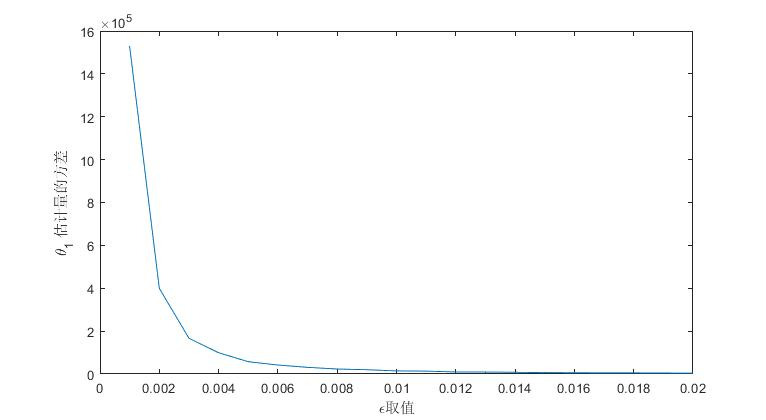
\includegraphics[scale=0.5]{fig3.1.jpg}
	\caption{\(\theta\)的第一个分量的估计量的方差随\(\epsilon\)变化曲线}
	\label{3.1}
\end{figure}

\begin{figure}[H]
	\centering
	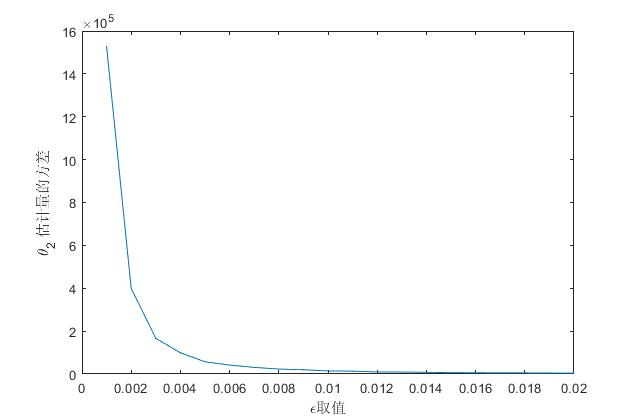
\includegraphics[scale=0.5]{fig3.2.jpg}
	\caption{\(\theta\)的第二个分量的估计量的方差随\(\epsilon\)变化曲线}
	\label{3.2}
\end{figure}

图3.1和图3.2显示了\(\theta\)的两个分量的估计量的方差随\(\epsilon\)变化曲线,随着\(\epsilon\)的减小,
\(\hat{\boldsymbol{\theta}}=(\mathbf{H}^T \mathbf{H})^{-1}\mathbf{H}^T\mathbf{z}\)
的估计性能逐渐变差。

\subsection*{*(3)如果已知\(\boldsymbol{\theta}\)中只有少部分分量非零,
	你认为选用哪种贝叶斯准则可以更好地处理该问题?为什么?}

由于\(\boldsymbol{\theta}\)中只有少部分分量非零,可以假设\(\boldsymbol{\theta}\)的各分量相互独立,
且服从均值为零的拉普拉斯分布,
即\(\boldsymbol{\theta} \sim \mathcal{L}(0,\sigma_{\theta}\mathbf{I})\),后验PDF为
\begin{align*}
	p(\boldsymbol{\theta})=\frac{1}{\sigma_{\theta}^P}
	\exp\left\{-\frac{1}{\sigma_{\theta}}\sum_{p=0}^{P-1}|\theta_p| \right\}
\end{align*}

利用\(p(\mathbf{z};\boldsymbol{\theta})\)可以得到联合概率密度函数

\begin{align*}
	p(\mathbf{z},\boldsymbol{\theta})
	 & =p(\mathbf{z}|\boldsymbol{\theta})p(\boldsymbol{\theta}) \\
	 & =\frac{1}{(2\pi \sigma_e^2)^{\frac{N}{2}}}
	\exp\left\{-\frac{1}{2\sigma_e^2} \left[\mathbf{z-H}\boldsymbol{\theta}\right]^T
	\left[\mathbf{z-H}\boldsymbol{\theta}\right]\right\}\cdot \frac{1}{\sigma_{\theta}^P}
	\exp\left\{-\frac{1}{\sigma_{\theta}}\sum_{p=0}^{P-1}|\theta_p| \right\}
\end{align*}

由上式很难求出\(p(\boldsymbol{\theta}|\mathbf{z})\)的解析形式。如果进行数值积分,后验PDF
\begin{align*}
	p(\boldsymbol{\theta}|\mathbf{z})=\frac{p(\mathbf{z}|\boldsymbol{\theta}p(\boldsymbol{\theta}))}
	{\int p(\mathbf{z|\boldsymbol{\theta}})p(\boldsymbol{\theta})d\boldsymbol{\theta}}
\end{align*}
中需要求关于\(\boldsymbol{\theta}\)的P维积分,十分困难,因此求最小均方估计存在难度。

可以使用最大后验概率准则来获得最大后验概率估计,即
\begin{align*}
	\hat{\boldsymbol{\theta}}=arg \underset{\boldsymbol{\theta}}{\max}
	p(\boldsymbol{\theta |\mathbf{z}})
\end{align*}
由于不需要计算边缘PDF,消除了积分运算,可以等价的表示为
\begin{align*}
	\hat{\boldsymbol{\theta}}=arg \underset{\boldsymbol{\theta}}{\max}p(\mathbf{z}|\boldsymbol{\theta })
	p(\boldsymbol{\theta})
\end{align*}
或
\begin{align*}
	\hat{\boldsymbol{\theta}}arg \underset{\boldsymbol{\theta}}{\max}=
	\left\{-\frac{1}{2\sigma_e^2} \left[\mathbf{z-H}\boldsymbol{\theta}\right]^T
	\left[\mathbf{z-H}\boldsymbol{\theta}\right]
	-\frac{1}{\sigma_{\theta}}\sum_{p=0}^{P-1}|\theta_p|\right\}
\end{align*}


\section{第四题}
\subsection*{什么情况下可以用线性最小均方估计?}

MMSE 估计量含有多重积分的计算,在实际实践中常因其计算量太大而难以实现,
而MAP 估计量涉及多维最大值求解的问题,尽管这些问题在联合高斯的假设下容易求得,
但是在一般情况下求解不简单,因此在无法做出高斯假设的情况下,就要使用其他方法。

LMMSE 是在保留 MMSE准则的条件下,限定估计量是线性的,来确定估计量。
LMMSE 依赖于随机变量的相关性,当数据和参数相关时,可以采用LMMSE。在已知被估计量的一阶矩和二阶矩,
可以采用线性最小均方估计。

\subsection*{如何理解递推线性最小均方估计的几何意义?}

递推LMMSE本质是将观测矢量\(z_n\)进行正交化,产生一组彼此不相关(垂直或者正交)的随机矢量,即新息
\(z[0],z[1]-\hat{z} [1|0],z[2]-\hat{z}[2|0,1],\dots \),新息是每个新增的观测值\(z(n)\)所贡献的新的信息。
这些新息组成了LMMSE,每增加一个数据相当于产生了新息,被估计量在这个新息的投影作为修正项对估计进行更新,
从而增加了估计量的新息。

\subsection*{考虑如下观测模型
	\begin{align*}
		z_n=A^k+w_n,n=0,1,\dots,N-1
	\end{align*}
	其中\(A\sim \mathcal{N}(0,\sigma^2_A)\),观测噪声\(w_n\overset{i,i,d}{\sim}\mathcal{N}(0.\sigma^2)\)
	且与A相互独立。}
\subsection*{(1)若\(k=2,N=1\),试考虑A的线性最小均方估计并分析你的结果。}

若k=2,N=1,观测模型为\(z_0=A^2+w_0\),根据线性最小均方估计的计算公式,得
\begin{align*}
	\hat{A}=E(A)+C_{Az}C_{zz}^{-1}(z-E(z))
\end{align*}
分别计算得
\begin{align*}
	E(A)   & =0                             \\
	C_{Az} & =E[(A-E(A))(z_0-E(z))]=E[Az_0] \\
	       & =E(A(A^2+\omega_0))=E(A^3)=0   \\
	C_{zz} & =E[(z_0-E(z))(z_0-E(z))]       \\
	       & =E[z_0^2-E^2(z)-2z_0E(z)]      \\
	       & =2\sigma_A^4+\sigma^2
\end{align*}
代入得
\begin{align*}
	\hat{A}=0
\end{align*}

可见计算的A的线性最小均方估计为0,与观测数据无关,这是因为A与观测数据不是线性关系导致的.

\subsection*{(2)若\(k=1,N>1\),试考虑A的递推线性最小均方估计并分析其性能。}

此时观测模型变为
\begin{align*}
	z_k=A+\omega_k,n=0,1,\dots,N-1
\end{align*}
根据递推线性最小均方估计的求解过程,首先基于第一个观测量\(z[0]\)求\(\hat{A}[0]\),其中
\(\hat{A}[0]\)为A在\(z[0]\)上的投影

\begin{align*}
	\hat{A}[0]=\left( A,\frac{z_0}{|z_0|}\right)\frac{z_0}{|z_0|}=\frac{E(Az_0)}{z_0^2}z_0
	=\frac{\sigma_A^2}{\sigma_A^2+\sigma^2}z_0
\end{align*}

之后求出基于\(z[0]\)的\(z[1]\)的LMMSE估计量得到\(\hat{z}[1|0]\):
\begin{align*}
	\hat{z}[1|0]=\left( z_1,\frac{z_0}{|z_0|}\right)\frac{z_0}{|z_0|}=\frac{E(z_1 z_0)}{z_0^2}z_0
	=\frac{\sigma_A^2}{\sigma_A^2+\sigma^2}z_0
\end{align*}
之后得到新息\(z[1]-\hat{z}[1|0]\):
\begin{align*}
	\widetilde{z}_1=z[1]-\hat{z}[1|0]=z_1-\frac{\sigma_A^2}{\sigma_A^2+\sigma^2}z_0
\end{align*}
将A基于新息的LMMSE估计量\(\Delta\hat{A}[1]\)加到\(\hat{A}[0]\)上,得到\(\hat{A}[1]\):
\begin{align*}
	\Delta\hat{A}[1]=\left(A,\frac{\widetilde{z}_1}{|\widetilde{z}_1|}\right)
	\frac{\widetilde{z}_1}{|\widetilde{z}_1|}=\frac{E(A\widetilde{z}_1)}{E(\widetilde{z}_1^2)}\widetilde{z}_1
\end{align*}
令\(K[1]=\frac{E(A\widetilde{z}_1)}{E(\widetilde{z}_1^2)}\),得到
\begin{align*}
	K[1]       & =\frac{E(A\widetilde{z}_1)}{E(\widetilde{z}_1^2)}=\frac{\sigma_A^2}{2\sigma_A^2+\sigma^2} \\
	\hat{A}[1] & =\hat{A}[0]+\Delta\hat{A}[1]=\hat{A}[0]+K[1]\widetilde{z}_1
\end{align*}
根据新的观测量类推,最终结果为:
\begin{align*}
	\hat{A}[N]=\hat{A}[N-1]+\Delta\hat{A}[N]=\hat{A}[N-1]+K[N](z_n-\hat{z}[n|0,1,\dots,n-1])
\end{align*}
因为\(z[N]\)与以前的样本是不相关的,所以
\begin{align*}
	\hat{A}[N-1] & =\hat{z}[n|0,1,\dots,n-1]            \\
	\hat{A}[N]   & =\hat{A}[N-1]+K[N](z_n-\hat{A}[N-1])
\end{align*}
其中
\begin{align*}
	K[N]=\frac{Bmse(\hat{A}[N-1])}{Bmse(\hat{A}[N-1])+\sigma^2}
\end{align*}

起始值:
\begin{align*}
	\hat{A}[0]=\frac{\sigma^2_A}{\sigma^2_A+\sigma^2}z_0
\end{align*}

性能分析:
估计量的均方误差为
\begin{align*}
	Bmse(\hat{A}[N])=(1-K[N])Bmse(\hat{A}[N-1])=\frac{\sigma_A^2\sigma^2}{(N+1)\sigma^2_A+\sigma^2}
\end{align*}

可见随着估计量数目的增多,估计量的均方误差不断减小,可知非贝叶斯估计时均方误差为\(\frac{\sigma^2}{N}\),
非贝叶斯估计的均方误差始终大于贝叶斯估计的均方误差,可见由于先验信息的引入,估计精度被有效改善。

\bibliography{books}
\end{document}